\chapter{Tiempo de Retorno Energético  de Sistemas
  Fotovoltaicos}
\label{cha:LCA}


\section{Introducción}

Para conseguir que un sistema generador de energía funcione como tal,
es necesario el empleo de diferentes técnicas que a su vez demandan el
consumo de diferentes fuentes de energía. Así, a lo largo de su ciclo
de vida, además de producir energía y diferentes residuos, un sistema
generador requerirá el empleo de energía para la fabricación de sus
componentes, el tratamiento del terreno en el que será ubicado, el
transporte e instalación de los equipos que lo forman, el combustible
necesario para su funcionamiento, la reposición de los equipos que
agotan su ciclo, etc.

El Análisis de Ciclo de Vida --\emph{Life Cycle Assesment} (LCA)--
tiene como objetivo documentar y analizar los impactos que un sistema
provoca sobre su entorno desde su producción hasta su desmantelamiento
y reciclaje (la terminología inglesa utiliza expresiones como \emph{from
cradle to grave}, de la cuna a la tumba, para expresar este concepto).
% La figura \ref{fig:Flujo-de-energia} resume visualmente este enfoque
% aplicado a un SFCR.

Para la aplicación de este enfoque al estudio del impacto \emph{energético}
de un SFCR se estudian tres fuentes de información: 

\begin{itemize}

\item Inventarios de Ciclos de Vida (\emph{Life Cycle Inventory,} LCI) de
los procesos empleados para implementar un SFCR. A partir de estos
LCIs es posible estimar el impacto energético asociado.

\item Radiación global del lugar en el que el SFCR va a desempeñar sus funciones

\item Características técnicas de los diferentes componentes del SFCR que
permitan estimar la energía producida a lo largo de toda su vida útil. 

\end{itemize}

En el capítulo \ref{cha:SFCR} se han descrito los métodos que se deben
emplear para estimar la producción energética de un SFCR a partir de
la radiación global y las características de los principales equipos
de un SFCR. Este capítulo analiza el impacto energético de los métodos
de producción de los principales componentes de un SFCR.  De esta
manera se obtendrá información del flujo de energía necesario para el
buen funcionamiento de un SFCR, y se establecerán comparativas y
análisis sobre la influencia de las diferentes técnicas de seguimiento
en el rendimiento energético.

Cabe reseñar la existencia de numerosos estudios previos que han
analizado con diversos enfoques el impacto ambiental de los sistemas
fotovoltaicos.  En general, pueden establecerse dos grupos
principales: el de aquellos análisis que ponen el acento en el módulo
fotovoltaico, dedicando una atención secundaria al resto de equipos; y
el de los que recogen las cifras estimadas por otros para cuantificar
el impacto del módulo, y detallan la implicación de los otros equipos
que componen el sistema.  Como representación del primer grupo cabe
destacar las referencias \cite{Alsema2000, Alsema.Wild-Scholten2006,
  Wild-Scholten2013}, aunque la lista que compone este conjunto es
amplia y diversa en resultados \cite{Keoleian.Lewis1997},
\cite{Knapp.Jesterm2001, Jungbluth2005, Dones.Frischkenecht1998}. En
el segundo grupo es referente el estudio realizado por
\cite{Mason.Ftherakis.ea2006}, aunque otros estudios menos recientes
contienen comparativas interesantes \cite{Meier2002,
  Krauter.Ruether2004,Frankl.Masini.ea1998}. No obstante, es
destacable que ninguno de los trabajos reseñados analiza el ciclo de
vida de sistemas de seguimiento.

% \begin{figure}[H]
% \begin{centering}
% 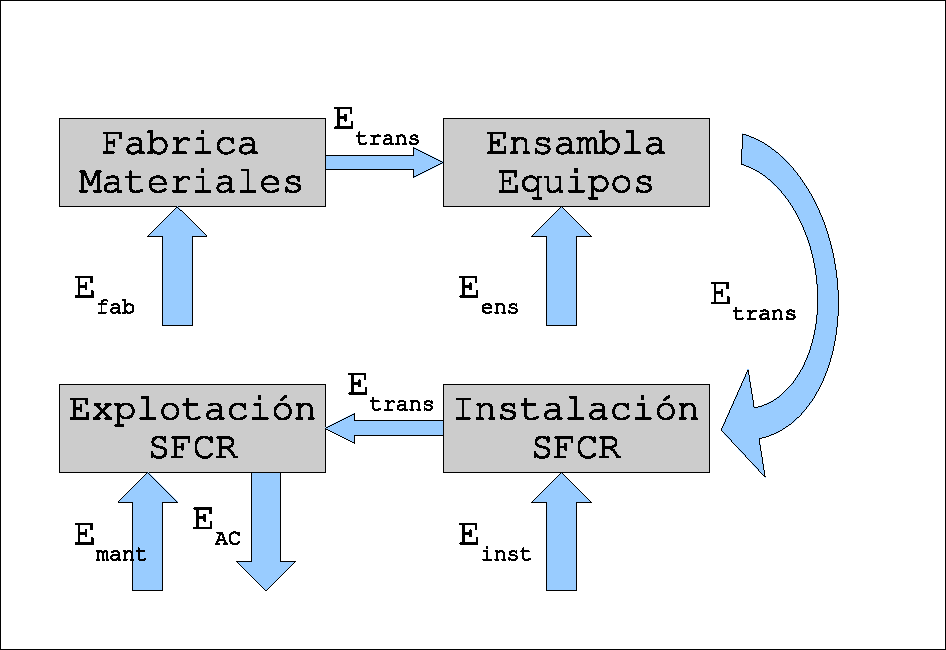
\includegraphics[width=0.9\textwidth]{../figs/LCAFlujo}
% \end{centering}
% \caption[Flujo de energía en la ejecución y explotación de un
% SFCR]{\label{fig:Flujo-de-energia}Flujo de energía en la ejecución y
%   explotación de un SFCR. No se ha incluido la fase de
%   desmantelamiento ni reciclaje de materiales. $E_{fab}$ representa la
%   energía empleada en la fabricación de los materiales, $E_{ens}$ la
%   energía empleada en el ensamblaje de los equipos principales a
%   partir de los materiales,$E_{inst}$ es la energía empleada en la
%   ejecución del SFCR, $E_{mant}$ es la energía empleada en el
%   mantenimiento del sistema, $E_{trans}$ es la energía empleada en el
%   transporte entre las diferentes fases del proyecto, y finalmente
%   $E_{AC}$ es la energía producida por el SFCR.}
% \end{figure}

\section{Métodos}


\subsection{Fronteras del Estudio}

La aplicación de un estudio del ciclo de vida energético a un sistema
exige la definición de las fronteras espaciales y temporales que
contienen los productos y procesos que formarán parte del
cálculo. Esta definición de fronteras permite establecer indicadores
útiles para la comparación con sistemas alternativos. En el caso que
nos ocupa, el objetivo es analizar el comportamiento de diferentes
técnicas de seguimiento a lo largo de su vida útil. Por tanto, las
fronteras dejarán fuera los componentes cuya elección y diseño
dependen de condiciones coyunturales (por ejemplo, normativa local de
conexión a red en Media Tensión), y en todo caso, debieran ser
adoptados por el diseñador independientemente de la técnica de
seguimiento adoptada. Por simplificarlo con una etiqueta, diremos que
la frontera es la Baja Tensión (BT). 

Así, nuestro LCI incluirá la energía empleada en la fabricación y
transporte de los módulos fotovoltaicos, cableado de BT, inversores,
estructura de soporte y cimentaciones, y no se tendrán en cuenta los
Centros de Transformación y Lineas de Media Tensión. Otros procesos
incluidos dentro de la frontera de Baja Tensión se descartan por su
escasa influencia en la contabilidad global: protecciones de BT, mano
de obra, equipos accesorios de obra, sistemas de comunicaciones,
documentación y tareas de mantenimiento.

\subsection{Reposición de Equipos}


A lo largo de la vida útil del sistema (por ejemplo, 30 años) ciertos
componentes deberán ser reemplazados para garantizar la disponibilidad
del sistema como generador. El impacto energético asociado deberá
ser incluido en el análisis, teniendo en cuenta la tasa de fallos
asociado a cada componente, y por tanto la frecuencia de reposición
de equipos o tareas de reparación necesarias. 

La tasa de fallos de un módulo fotovoltaico es muy baja --en general,
los fabricantes aportan garantías que superan los 20 años--, y
consecuentemente el impacto energético es despreciable en el cálculo
global. 

Los inversores se caracterizan por tasas de fallos más elevadas,
aunque en general debido a sus componentes electrónicos y no a las
etapas de potencia (puente de transistores IGBTs y transformador, que
son los partes del inversor que más contribuyen a su impacto
energético). Actualmente, es frecuente encontrar inversores diseñados
para evitar la sustitución total del equipo cuando la avería se ha
producido fuera de las etapas de potencia, disminuyendo
considerablemente el impacto energético durante el ciclo de vida del
sistema. 

El cableado, estructura metálica y cimentación se caracterizan por su
estabilidad: garantizar su disponibilidad solo exige actuaciones
menores de mantenimiento sin influencia relevante en el cálculo
energético (por ejemplo, repaso de soldaduras en la estructura, o
aplicación de empalmes en cableado). 

En resumen, el impacto energético asociado a la reposición de equipos
para garantizar la disponibilidad del sistema no es relevante en el
cálculo global.

\subsection{Contribución Energética de Procesos y Productos}


Una vez definida la frontera que delimita el estudio, comienza la
tarea nada evidente de asignar valores unitarios de energía a cada
proceso y producto. Como se señaló en la introducción, no son pocos
los estudios que informan de conjuntos de valores para sistemas
fotovoltaicos.  La bibliografía reseñada provee de detallada
información sobre el principal componente, el módulo fotovoltaico,
resolviendo sin tanta profundidad los impactos de los otros
componentes englobados en el \emph{Balance of System} o \emph{Resto
  del Sistema}).  En general, todos los documentos trabajan con
sistemas estáticos sin ninguna referencia relevante a técnicas de
seguimiento.

Como se verá en la relación de resultados, la contribución de este
\emph{resto del sistema} ronda la cuarta parte del total de la energía
invertida, valor en absoluto desdeñable. No obstante, todos los
valores deben tratarse con la debida precaución, tanto en lo relativo
a módulos fotovoltaicos como al resto del sistema: la variedad de
materiales y procedimientos tecnológicos son difícilmente
cuantificables con cifras caracterizadas simultáneamente por su
exactitud y generalidad, máxime cuando las reticencias impuestas por
la confidencialidad industrial contribuyen al ruido en la
información. Por ejemplo, \cite{Alsema2000} realiza una revisión de
estimaciones publicadas en la que encuentra valores en un rango
comprendido entre $\SI{5300}{\mega\joule\per\squared\meter}$ y
$\SI{16500}{\mega\joule\per\squared\meter}$ para la fabricación de
módulos de silicio monocristalino. Es más, a pesar de realizar un
análisis comparativo para conseguir la mejor estimación, que este
autor cifra en $\SI{5700}{\mega\joule\per\squared\meter}$, concluye
que la incertidumbre no es menor del 40\%. De ahí que los resultados
que se obtengan serán meramente indicativos y útiles en el contexto de
la comparativa enunciada.

Hechas estas aclaraciones se enumeran las fuentes de información de
las que nos hemos servido para obtener valores unitarios de energía
de procesos y productos. Téngase en cuenta que todo el inventario
recopila cifras de energía primaria. 

Según la referencia \cite{Alsema.Wild-Scholten2006}, la energía
primaria empleada en la fabricación de los módulos fotovoltaicos de
silicio monocristalino es de
$\SI{5200}{\mega\joule\per\squared\meter}$, con el desglose recogido
en la tabla \ref{tab:ContribucionEnergetica}. El documento de esta
referencia es el resultado de un proyecto colaborativo, en el que
numerosas empresas e investigadores han aunado esfuerzos para
recopilar LCIs que representan el estado actual de la tecnología de
producción de módulos de silicio cristalino. Se debe señalar que la
energía empleada en el marco de aluminio ha sido estimada a partir de
\cite{Baird.Alcorn.ea1997} teniendo en cuenta la proporción de
aluminio reciclado empleado en el proceso de la empresa Isofotón.

\begin{table}[p]
  \caption[Contribución energética de cada fase en el proceso de fabricación
  de un módulo fotovoltaico de silicio monocristalino.]{\label{tab:ContribucionEnergetica}Contribución energética
    de cada fase en el proceso de fabricación de un módulo fotovoltaico
    de silicio monocristalino \cite{Alsema.Wild-Scholten2006}.}

\centering{}%
\begin{tabular}{cc}
\toprule
Fase & Contribución (\%)\tabularnewline
\midrule
Marco & 5\tabularnewline
\midrule
Ensamblado de Módulo & 7,25\tabularnewline
\midrule
Producción de célula & 9,05\tabularnewline
\midrule
Lingote y Oblea & 47,1\tabularnewline
\midrule
Aprovisionamiento de Silicio & 31,6\tabularnewline
\bottomrule
\end{tabular}
\end{table}


La energía empleada en la fabricación de inversores ha sido calculada
a partir de la tabla II de \cite{Alsema.Wild-Scholten2006} adaptada a
inversores de diferentes tamaños y fabricantes, mientras que la
empleada en la fabricación del cableado (cobre y aluminio),
estructuras metálicas (acero galvanizado) y cimentaciones (hormigón y
acero) ha sido calculada a partir de \cite{Baird.Alcorn.ea1997}. El
cálculo de energía empleado en el transporte de todos los equipos y
materiales se ha realizado a partir de las cifras publicadas en
\url{http://en.wikipedia.org/wiki/Fuel_efficiency_in_transportation}.

Para componer el resultado total por sistema se han utilizado valores
promedio resultantes de proyectos diseñados y ejecutados por Isofotón
en las modalidades de seguimiento a doble eje, horizontal y estática.
Los parámetros recopilados de estos proyectos han sido la potencia del
generador e inversor, secciones y distancia de cableado, peso de acero
de estructura, volumen de hormigón y peso de acero en armado de
cimentación. La energía empleada en el transporte de los componentes
principales ha sido estimada con distancias medias entre las
localizaciones de los suministradores de equipos y las ubicaciones de
los diferentes proyectos. Los detalles de los proyectos, equipos
implicados y cálculos asociados están documentados en el artículo
\cite{Perpinan.Lorenzo.ea2009}.

\subsection{Métricas}

Una vez obtenidos los valores de energía empleada en el sistema
($E_{LCA}$) y energía producida por el mismo ($E_{ac}$) durante todo
el ciclo de vida, son de uso común diferentes métricas para comparar
diferentes tecnologías de generación. Las más frecuentes son las
denominadas \emph{eficiencia del ciclo de vida} y \emph{tiempo de
  recuperación de la energía empleada}, particularmente esta última
\cite{Meier2002, Keoleian.Lewis1997}:

\begin{itemize}
\item Eficiencia del ciclo de vida, que puede definirse de diversas
  formas:

  \begin{itemize}
  \item Ratio entre la producción neta del sistema respecto a la
    radiación incidente durante el ciclo de vida \cite{Keoleian.Lewis1997}:
    \begin{equation}
      \eta_{LCA}=\frac{E_{ac}-E_{LCA}}{G_{ef}}
      \label{eq:EfLCA}
    \end{equation}

  \item Ratio entre la producción del sistema respecto a la suma de
    energías que entran en el sistema (energía empleada durante su
    ciclo de vida y radiación incidente) \cite{Meier2002}:
    \begin{equation}
      \eta_{LCA}=\frac{E_{ac}}{E_{LCA}+G_{ef}}
      \label{eq:EfLCA2}
    \end{equation}

  \end{itemize}
\item Tiempo de recuperación de la energía empleada (\emph{Energy
    PayBack Time}, EPBT):
  \begin{equation}
    EPBT=\frac{E_{LCA}}{E_{ac}}
    \label{eq:EPBT}
  \end{equation}

\end{itemize}

En los análisis que involucran a sistemas de energía solar o eólica,
en los que el recurso no representa ningún coste energético, los
resultados aportados por la eficiencia de ciclo de vida son poco
significativos, y no aportan más información de la que puede aportar
el cálculo convencional de la eficiencia de conversión. Mucho más útil
es el uso del EPBT, y de ahí su mayor frecuencia de uso en todos los
estudios reseñados.  En este análisis se considerará exclusivamente
esta métrica como herramienta comparativa.


\subsection{La Cuestión del Mix Energético}

Para aquellas fases del proceso que utilizan energía eléctrica como
fuente principal, estas cifras de energía primaria dependen
fuertemente de los valores de eficiencia de conversión del sistema
energético donde se localizan las diferentes fases del proceso. Estos
valores se calculan a partir de la composición de fuentes energéticas
--el denominado mix energético-- variable por países y regiones. En
este estudio se ha supuesto una eficiencia de 0,31, representativo del
mix característico de la zona UCTE\footnote{La ``Unión para la
  Coordinación y Transmisión de la Electricidad'' es la asociación de
  operadores del sistema de transmisión en Europa continental, con el
  objetivo de coordinar los intereses de los operadores de 23 países
  europeos. Más información en UCTE \url{http://www.ucte.org/}.%
} \cite{Alsema.Wild-Scholten2006}.

El proceso de producción de un módulo fotovoltaico a partir de
polisilicio es mayoritariamente eléctrico (el 80\% de la energía
primaria se emplea en generar electricidad) y por tanto, olvidando
consideraciones geopolíticas, sería aconsejable localizar los centros
de fabricación en zonas con un alto valor de eficiencia de conversión
(por ejemplo, zonas con alta penetración de energía hidráulica, eólica
y solar). Desde el punto de vista medioambiental (por ejemplo, emisión
asociada de gases de efecto invernadero), el impacto de los sistemas
fotovoltaicos será tanto menor cuanto mayor la penetración de las
energías renovables en la red. 

De la misma manera, la energía eléctrica producida por el SFCR es
traducida a su valor de energía primaria teniendo en cuenta el
\emph{mix} energético de la localidad del sistema. En general, esta
ubicación está distante de las localidades donde se fabrican los
componentes del SFCR, lo que conduce a dos valores diferentes de
eficiencia de conversión del sistema eléctrico. Suponiendo constantes
los valores de energía eléctrica producida y empleada, en general se
obtendrán menores valores de EPBT ubicando los procesos de fabricación
en zonas con sistemas eléctricos muy eficientes (alta penetración de
hidráulica, eólica y solar) e instalando los correspondientes SFCR en
zonas con sistemas eléctricos poco eficientes (alta penetración de
generadores basados en fuentes fósiles) \cite{Krauter.Ruether2004}.


% \section{Resultados}

% Combinando estas fuentes de información se compone la tabla
% \ref{tab:ResultadosLCA}.  Todas las cifras son valores de energía
% primaria ($MJ_{p}$) normalizados a la potencia nominal del generador
% (kWp). Como métrica de análisis se utilizará el EPBT. 
% Se han generado mapas de EPBT para sistemas estáticos, eje horizontal
% Norte-Sur y seguimiento a doble eje . También se incluyen gráficas
% tipo ``box-plot'' para representar la mediana y primer y tercer
% cuartiles del EPBT para todo el rango de latitudes. Estos gráficos
% se han generado sin realizar interpolación espacial. Por último, se
% han incluido dos gráficos de dispersión para representar el EPBT frente
% a la radiación anual en el plano horizontal para las tres tecnologías,
% y para la comparativa entre doble eje y eje horizontal. Todas estas
% figuras se recogen en el apéndice \ref{cha:MapasLCA}.


\section{Resultados}


Combinando estas fuentes de información se compone la tabla
\ref{tab:CantidadComponentes}.  Todas las cifras son valores de
energía primaria ($MJ_{p}$) normalizados con la potencia nominal del
generador (kWp).

\begin{table}[p]
  \caption[Cuantificación de los componentes principales de una planta
  fotovoltaica.]{Cuantificación de los componentes principales de una
    planta fotovoltaica. Todas las cantidades están referidas a una potencia de generador FV
    de 1 kWp.}
  \label{tab:CantidadComponentes}

  \centering{}%
  \begin{tabular}{>{\centering}m{25mm}>{\raggedleft}m{15mm}>{\raggedleft}m{17mm}>{\raggedleft}m{15mm}>{\raggedleft}m{17mm}>{\raggedleft}m{15mm}>{\raggedleft}m{17mm}}
    \toprule 
    & \multicolumn{2}{c}{Doble Eje} & \multicolumn{2}{c}{Eje
      Horizontal N-S} & \multicolumn{2}{c}{Estático}\tabularnewline
    Componente & ($MJ_{p}/kWp$) & (\%) & ($MJ_{p}/kWp$) & (\%) & ($MJ_{p}/kWp$) & (\%)\tabularnewline
    \midrule 
    Módulo & 41\,819 & 69,54\% & 41\,819 & 78,67\% & 41\,819 & 81,99\%\tabularnewline
    \midrule 
    Estructura de Soporte & 9\,329 & 15,51\% & 6\,108 & 11,49\% & 4\,459 & 8,74\%\tabularnewline
    \midrule 
    Mecanismos de seguimiento & 248 & 0,41\% & 58 & 0,11\% & 0 & 0,00\%\tabularnewline
    \midrule 
    Cimentación (acero) & 3\,371 & 5,61\% & 1\,536 & 2,89\% & 0 & 0,00\%\tabularnewline
    \midrule 
    Cimentación (hormigón) & 2\,445 & 4,07\% & 1\,281 & 2,41\% & 2\,352 & 4,61\%\tabularnewline
    \midrule 
    Transporte & 1\,339 & 2,23\% & 900 & 1,69\% & 1\,037 & 2,03\%\tabularnewline
    \midrule 
    Inversor & 1,091 & 1,81\% & 1\,091 & 2,05\% & 1\,091 & 2,14\%\tabularnewline
    \midrule 
    Cableado & 497 & 0,83\% & 364 & 0,68\% & 248 & 0,49\%\tabularnewline
    \midrule 
    Total & 60\,140 & 100\% & 53\,157 & 100\% & 51\,005 & 100\%\tabularnewline
    \bottomrule
  \end{tabular}
\end{table}


\subsection{Energía Requerida}


Según la tabla \ref{tab:ResultadosLCA}, aproximadamente tres cuartas
partes de la energía empleada en las fases de fabricación y ejecución
del sistema recaen en el generador fotovoltaico. En segundo lugar
de importancia destaca la energía dedicada a la estructura de soporte
y su cimentación. Debido a los requerimientos de carga de viento de
las estructuras de seguidores de doble eje (altura de 10 metros, gran
superficie expuesta, único punto de apoyo, etc.), esta contribución
es considerablemente superior a la necesaria para sistemas estáticos
--una cuarta parte del total, aproximadamente el doble que lo necesario
en un sistema estático. Sin embargo, los sistemas de seguimiento horizontal
dedican a estas partidas valores de energía similares a los sistemas
estáticos, porque la estructura descansa sobre un eje horizontal a
baja altura del terreno, con apoyos distribuidos que reducen las necesidades
de cimentación respecto a los seguidores de doble eje. La importancia
del resto de partidas es secundaria. Merece la pena destacar que,
a pesar de ser necesario emplear cantidades superiores de cable en
plantas de seguimiento a doble eje --debido a su mayor ocupación de
terreno por sombreado mutuo--, la influencia final es mínima en las
tres tipologías.

\subsection{EPBT}

La tabla \ref{tab:ResultadosLCA} recoge el resumen de distribución de
valores del EPBT para los distintos sistemas considerados en las
condiciones de radiación y latitud de Europa. Estos valores están
representados en las figuras \ref{EPBT2xBoxPlot},
\ref{EPBTHorizBoxPlot} y \ref{EPBTEstBoxPlot}.

Tal y como ya han señalado otros autores, durante su vida útil un
sistema fotovoltaico es capaz de devolver varias veces la energía que
ha sido empleada en él. Las figuras \ref{EPBT2xBoxPlot},
\ref{EPBTHorizBoxPlot} y \ref{EPBTEstBoxPlot} muestran un conjunto de
valores de EPBT que se encuentran, para las condiciones de Europa, en
un rango entre 2 y 5 años, dependiendo del modo de seguimiento y la
latitud, lo que implica que un SFCR sería capaz de entregar entre 6 a
15 veces la energía empleada, suponiendo una vida útil de 30
años. Estas cifras concuerdan con las presentadas en la bibliografía
reseñada.

\begin{table}[p]

  \caption{\label{tab:ResultadosLCA}Resumen estadístico de los valores
    de EPBT de sistemas estáticos y de seguimiento para la región
    geográfica comprendida entre $-10^{\circ}$ y $10^{\circ}$ de
    longitud, y $30^{\circ}$ a $45^{\circ}$ de latitud.}


  \centering{}%
  \begin{tabular}{ccccccc}
    \toprule 
    EPBT & Min & Primer Cuartil & Mediana & Media & Tercer Cuartil & Max\tabularnewline
    \midrule 
    Doble Eje & 2,1 & 2,4 & 2,6 & 2,7 & 2,82 & 4,34\tabularnewline
    \midrule 
    Horizontal N-S & 2,3 & 2,65 & 2,88 & 3 & 3,17 & 4,9\tabularnewline
    \midrule 
    Estático & 2,68 & 3 & 3,22 & 3,3 & 3,45 & 4,8\tabularnewline
    \bottomrule
  \end{tabular}
\end{table}



\begin{figure}[p]
\begin{centering}
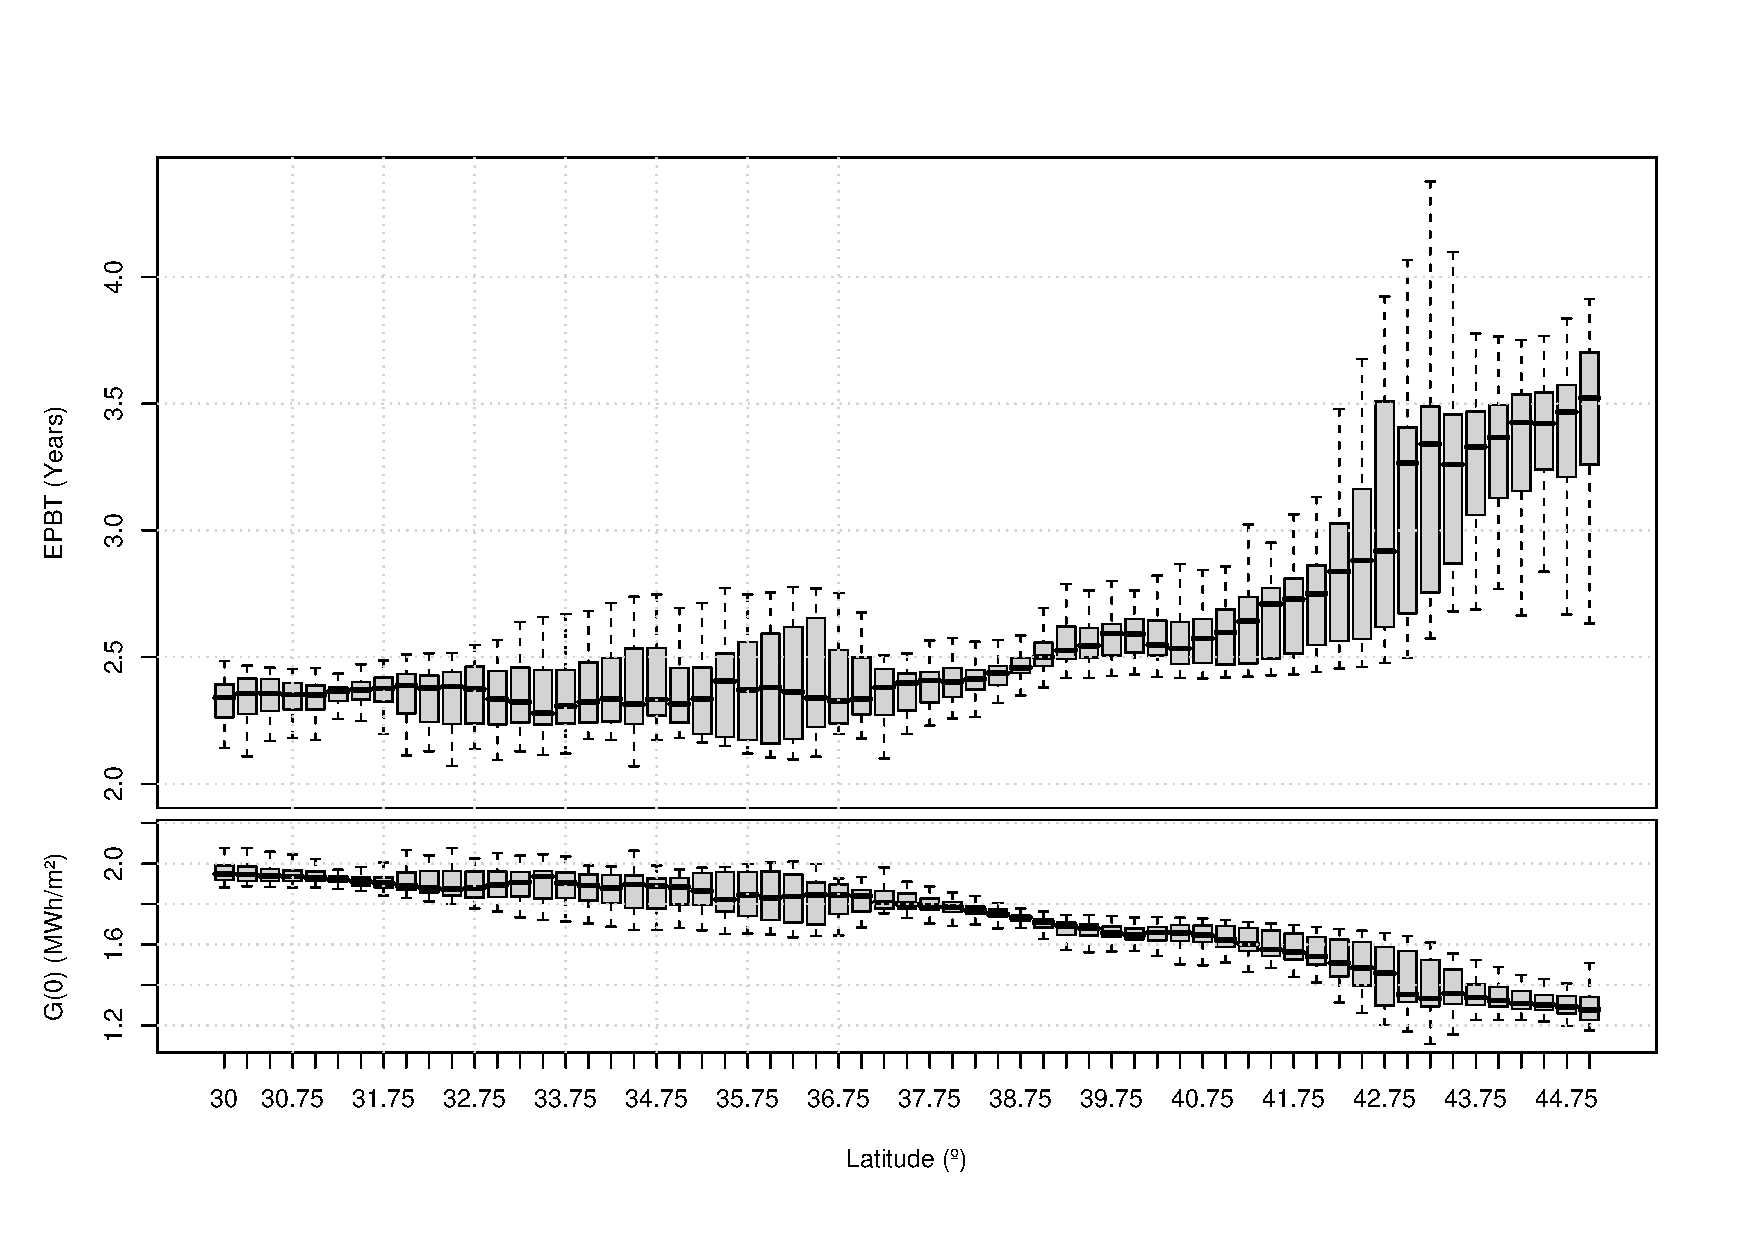
\includegraphics[height=0.38\textheight]{../figs/BoxPlotEPBTEuropa_SODA001}
\par\end{centering}

\caption{\label{EPBT2xBoxPlot}EPBT de un SFCR con seguimiento a doble
  eje para la región geográfica comprendida entre $-10^{\circ}$ y
  $10^{\circ}$ de longitud, y $30^{\circ}$ a $45^{\circ}$ de latitud.
  La figura inferior muestra los valores anuales de radiación global
  en el plano horizontal como referencia.}
\end{figure}


\begin{figure}[p]
\begin{centering}
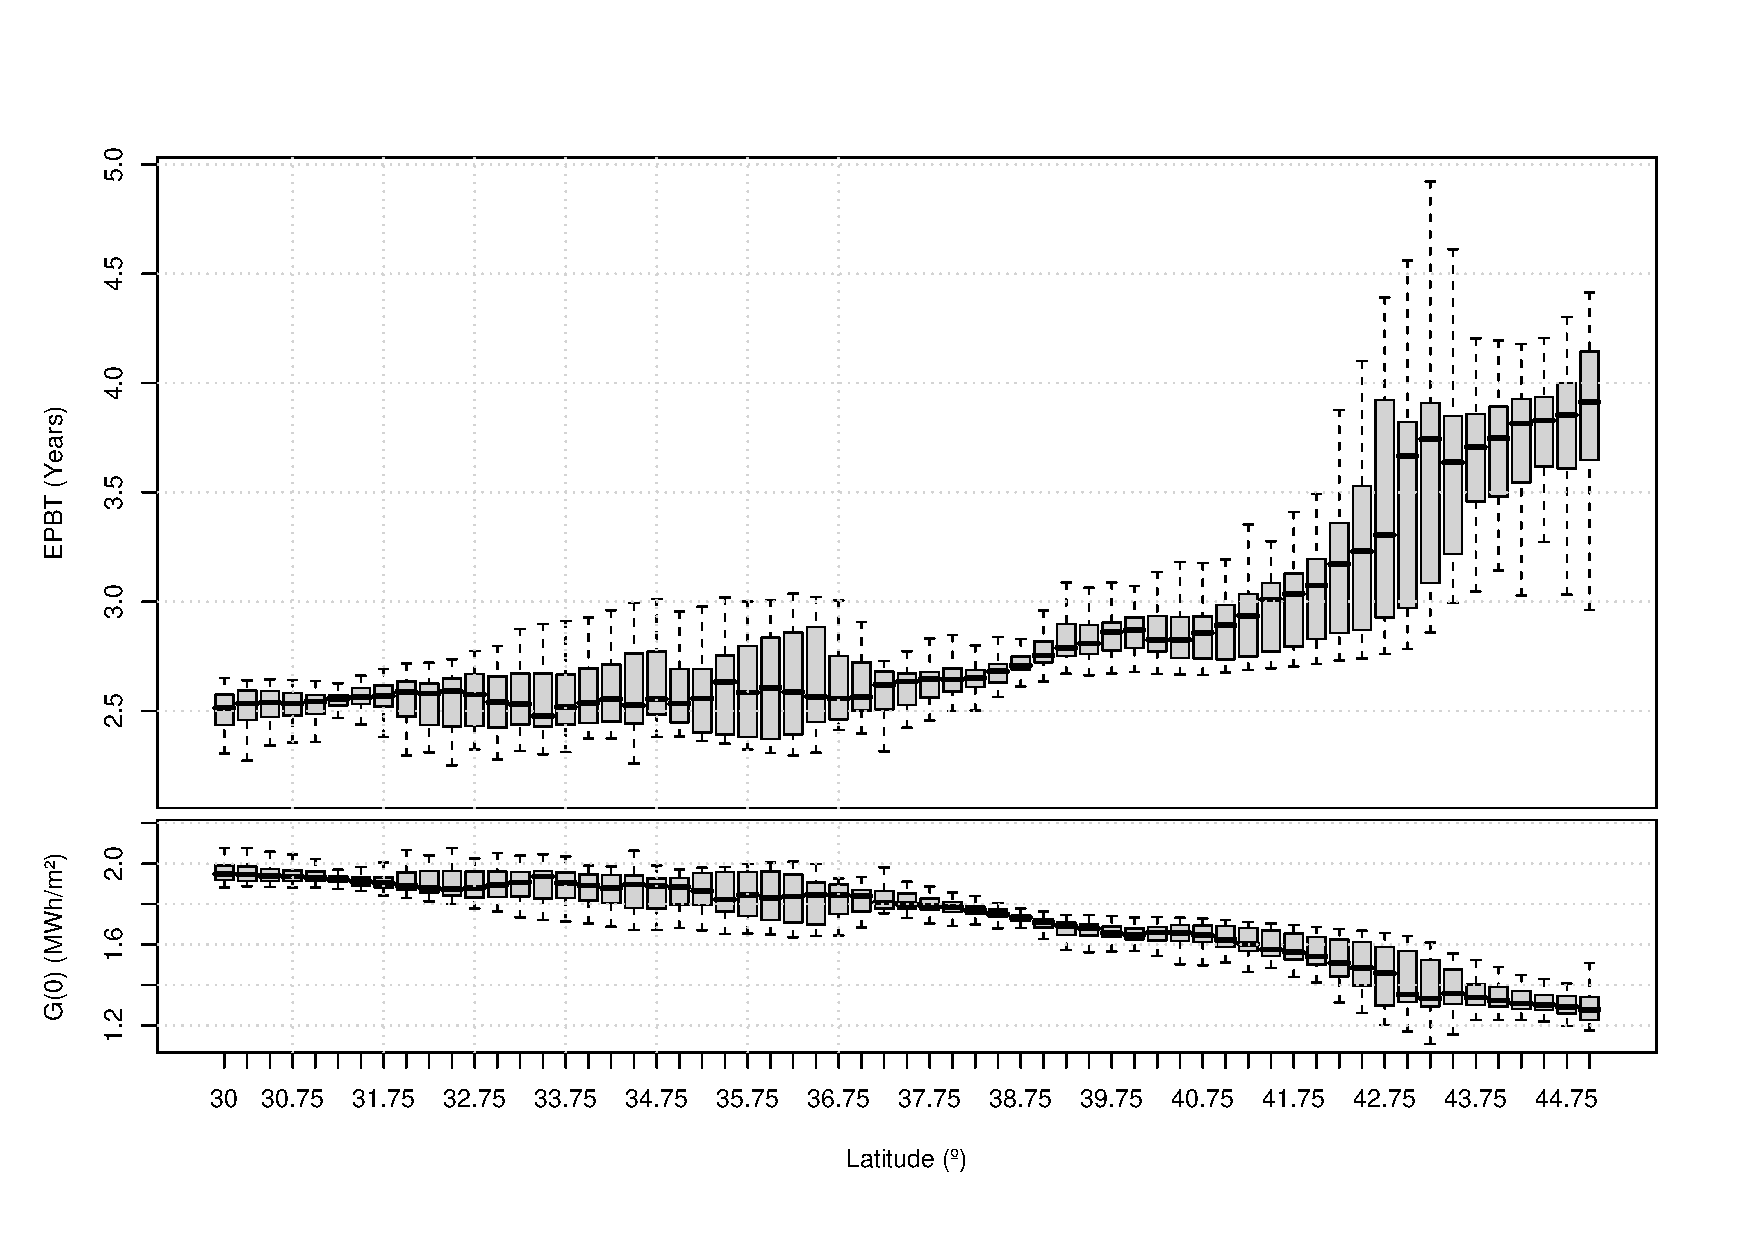
\includegraphics[height=0.38\textheight]{../figs/BoxPlotEPBTEuropa_SODA002}
\par\end{centering}

\caption{\label{EPBTHorizBoxPlot}EPBT de un SFCR con seguimiento
  horizontal N-S para la región geográfica comprendida entre
  $-10^{\circ}$ y $10^{\circ}$ de longitud, y $30^{\circ}$ a
  $45^{\circ}$ de latitud.  La figura inferior muestra los valores
  anuales de radiación global en el plano horizontal como referencia.}
\end{figure}


\begin{figure}[p]
\begin{centering}
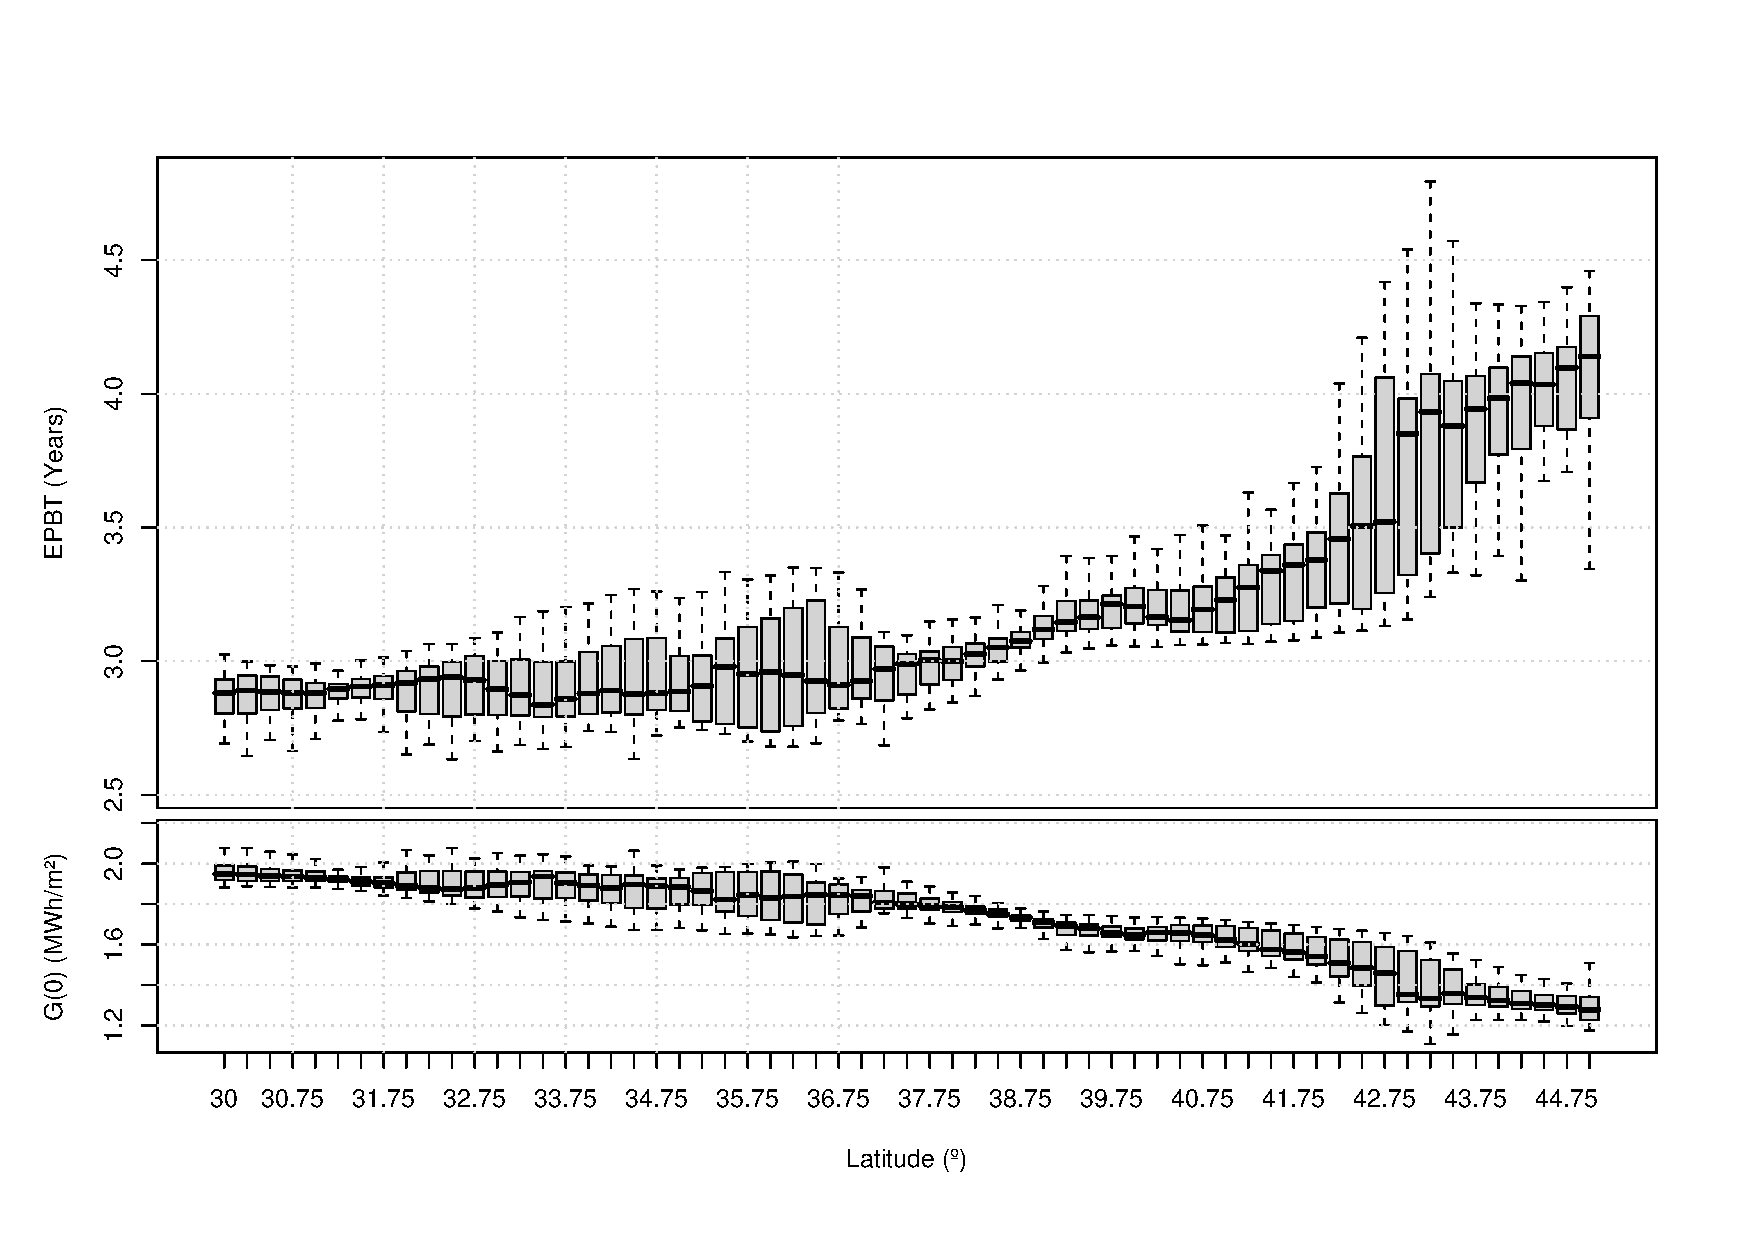
\includegraphics[height=0.38\textheight]{../figs/BoxPlotEPBTEuropa_SODA003}
\par\end{centering}

\caption{\label{EPBTEstBoxPlot}EPBT de un SFCR estático para la región
  geográfica comprendida entre $-10^{\circ}$ y $10^{\circ}$ de
  longitud, y $30^{\circ}$ a $45^{\circ}$ de latitud.  La figura
  inferior muestra los valores anuales de radiación global en el plano
  horizontal como referencia.}
\end{figure}



\subsection{Comparativa entre Sistemas}


Las figuras \ref{EPBTComparaBoxPlot} y \ref{EPBTComparaGh} comparan
los resultados para los tres sistemas y los relacionan con la
radiación. En general, en las condiciones de radiación y valores de
latitude de Europa y desde la perspectiva del EPBT, las dos
tecnologías de seguimiento son preferibles a los sistemas estáticos.

\begin{figure}[p]
\begin{centering}
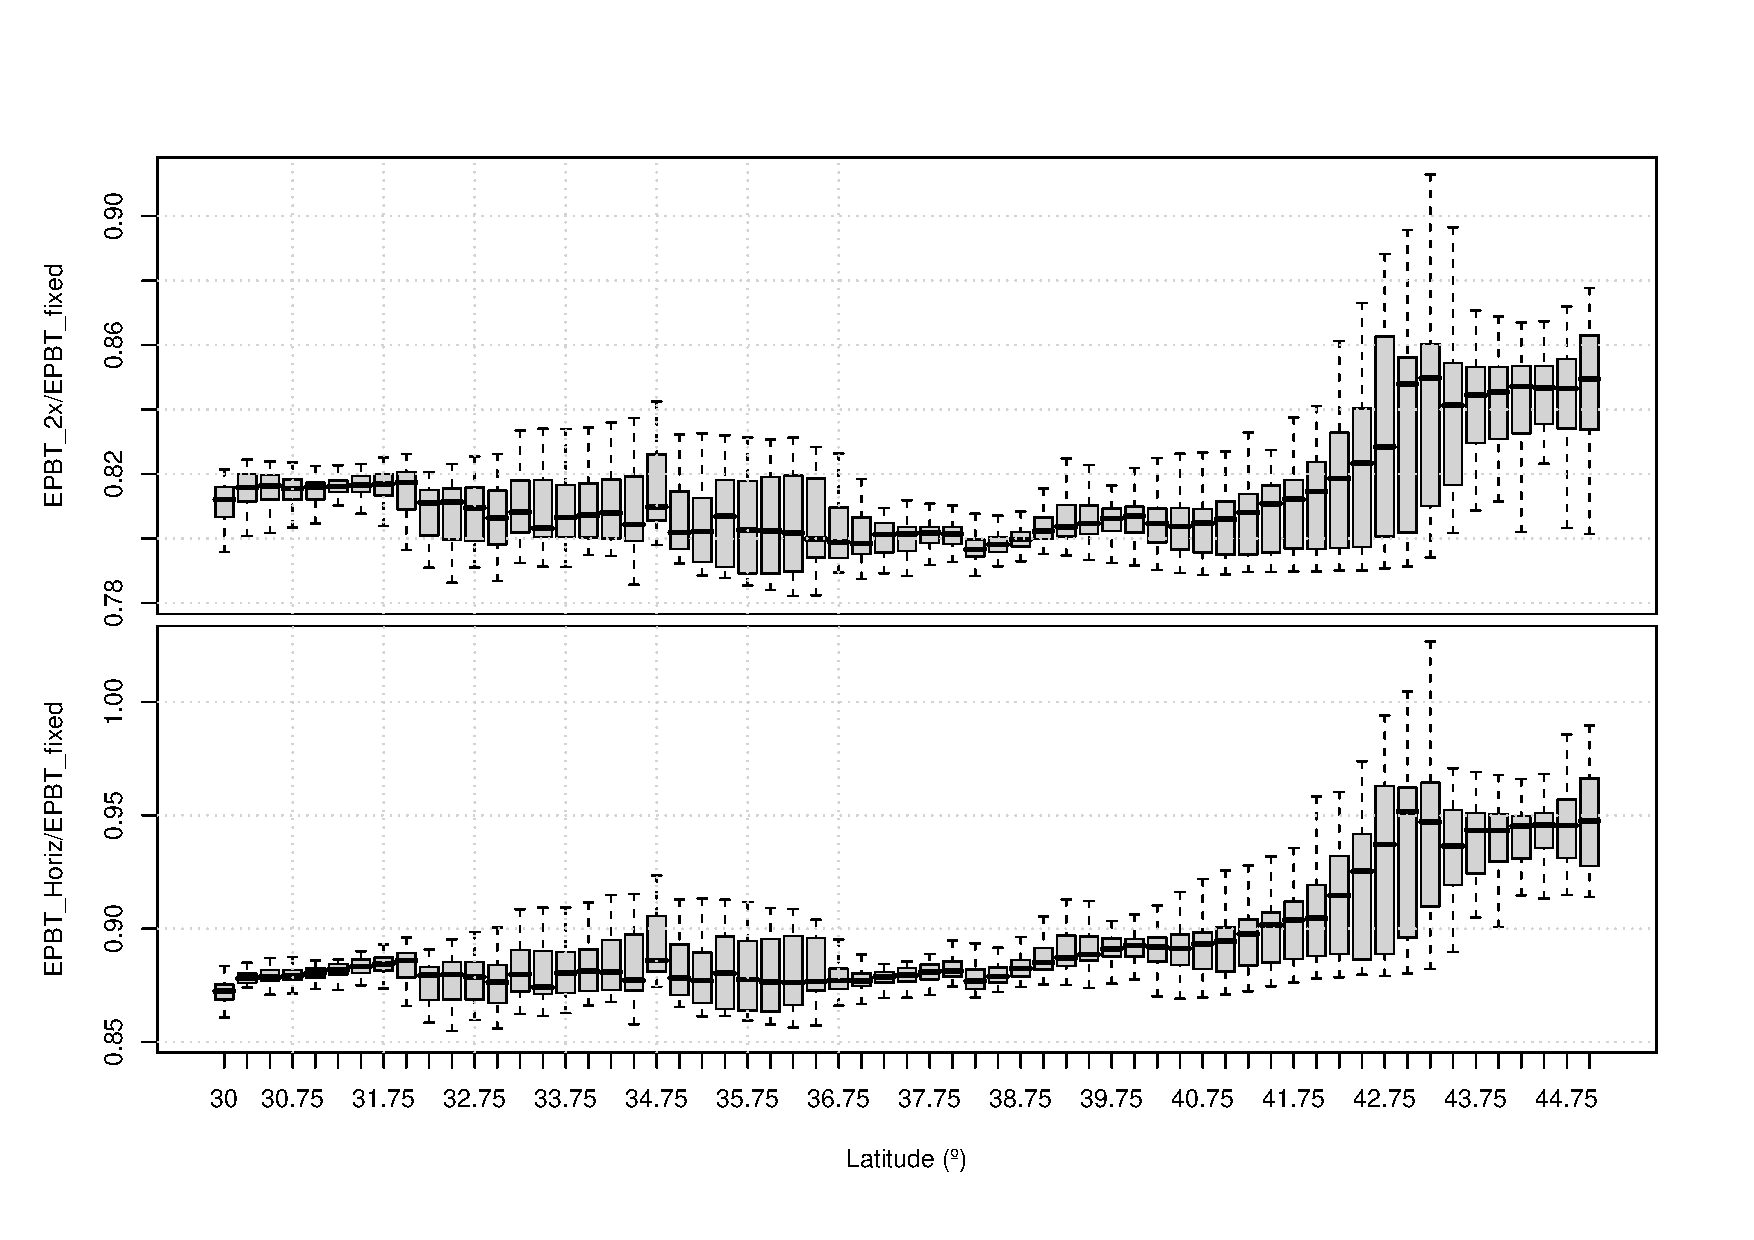
\includegraphics[height=0.38\textheight]{../figs/BoxPlotEPBTEuropa_SODA004}
\par\end{centering}

\caption{\label{EPBTComparaBoxPlot}Comparación entre los valores de
  EPBT de un sistema a doble eje y un estático (figura superior), y un
  sistema de seguimiento de eje horizontal N-S con un estático (figura
  inferior) para la región geográfica comprendida entre $-10^{\circ}$
  y $10^{\circ}$ de longitud, y $30^{\circ}$ a $45^{\circ}$ de
  latitud.}
\end{figure}


\begin{figure}[p]
\begin{centering}
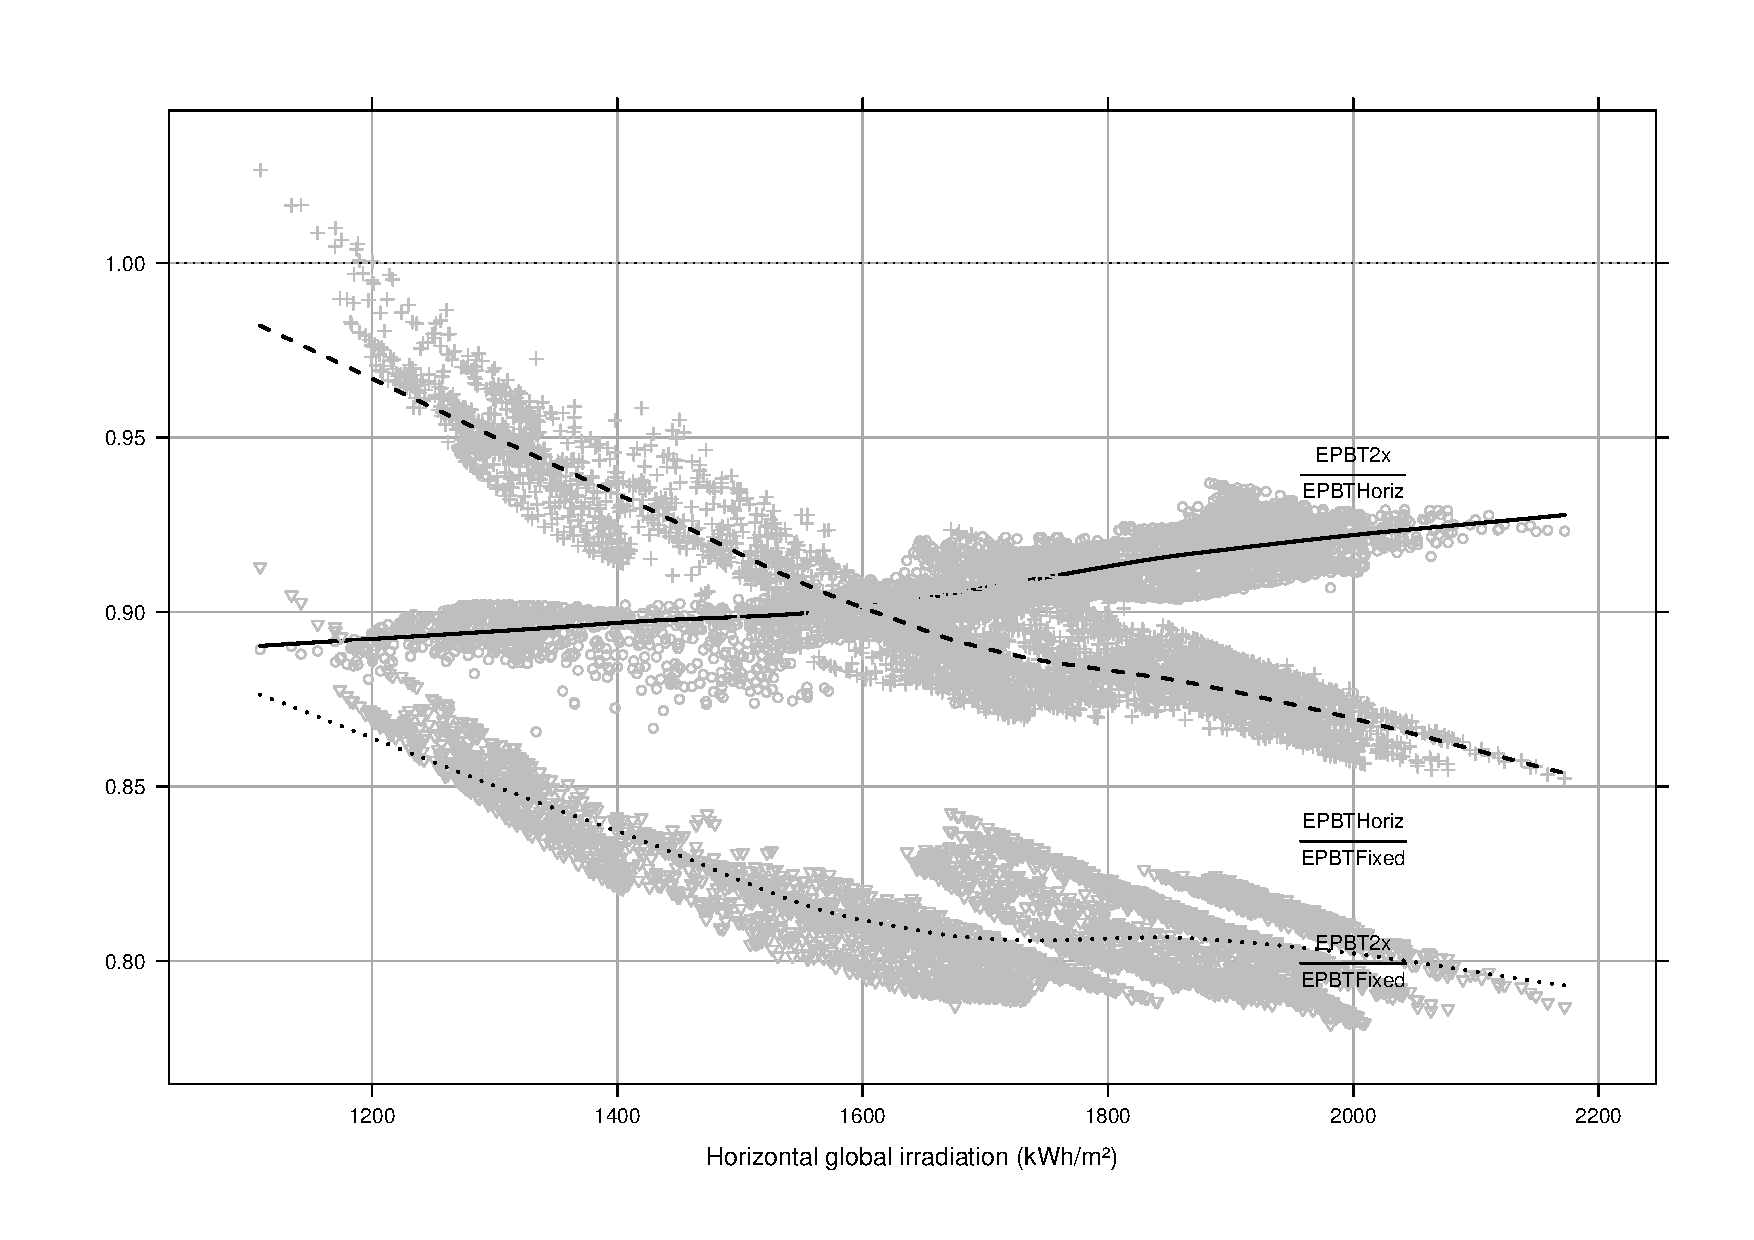
\includegraphics[height=0.38\textheight]{../figs/EPBTEuropavsGh2}
\par\end{centering}

\caption{\label{EPBTComparaGh}Comparación entre los EPBT de los
  diferentes sistemas frente a la radiación global en el plano
  horizontal en la región geográfica comprendida entre $-10^{\circ}$ y
  $10^{\circ}$ de longitud, y $30^{\circ}$ a $45^{\circ}$ de latitud.}
\end{figure}

La comparación entre las dos tecnologías de seguimiento debe
realizarse con más precaución. Tanto con la latitud como con la
radiación (figura \ref{EPBTComparaGh}) aparece una relación según la
cual el seguimiento a doble eje es preferible en latitudes altas y
radiaciones bajas. En toda la superficie en estudio el seguimiento a
doble eje ofrece valores de EPBT inferiores al seguimiento horizontal
con diferencias que oscilan entre el 9 y 15\%. Como ya se ha señalado
en los capítulos precedentes, la información de la que parten estos
cálculos (radiación efectiva, energía producida y energía empleada)
está sometida a una incertidumbre que puede ser incluso superior a
estas diferencias. 

Como se puede ver en las pendientes de la figura \ref{EPBTComparaGh},
el ratio $EPBT/G_{a}(0)$ es similar en todo el rango de radiación
horizontal para las dos tecnologías de seguimiento estudiadas, y algo
superior para estática. La menor energía empleada en una instalación
estática por su mayor simplicidad respecto a los sistemas de
seguimiento no compensa su peor productividad como generador.

Volviendo a la tabla \ref{tab:ResultadosLCA}, la gran importancia del
generador fotovoltaico aconseja emplear algo más de energía en el
resto de componentes para mejorar la productividad del sistema y
obtener el mayor rendimiento posible del componente más costoso
energéticamente. Tanto el seguimiento a doble eje como horizontal
siguen este camino, demandando mayor energía en estructura metálica,
cimentaciones y cableado, que se ve compensada ampliamente por la
mayor productividad del sistema. 

Otra forma de optimizar los valores de EPBT es la adoptada por los
sistemas de concentración, en los que el material activo es
sustancialmente reducido gracias al uso de componentes ópticos, cuyo
contenido energético es notablemente inferior. Además, las células
empleadas en estos sistemas suelen ofrecer cifras de eficiencia
superiores a las de los módulos convencionales, con el consiguiente
ahorro en material activo. A cambio, estos sistemas son ciegos a la
radiación difusa y requieren de un sistema de seguimiento con elevadas
prestaciones estructurales y de precisión. Dado el carácter
preindustrial de los equipos existentes hasta la fecha, y la falta de
experiencia de campo equivalente a la existente para módulos planos,
todos los análisis al respecto deben abordarse con cautela.  No
obstante, mencionaremos el estudio de \cite{Peharz.Dimroth2005}, que
arroja cifras de EPBT inferiores a un año para sistemas fabricados en
Alemania y explotados en Almería (alto índice de claridad), mostrando
que el mayor consumidor de energía del sistema es ahora el acero
estructural, con más del 40\% del total.

Cabe señalar que todas las comparativas que involucran a los sistemas
estáticos pierden su validez en el campo de la integración arquitectónica,
siempre y cuando el generador fotovoltaico sirva efectivamente como
elemento estructural del edificio, y no como mero recubrimiento. En
este caso, los requerimientos de acero estructural, aluminio y hormigón
para cimentación pueden reducirse en gran medida si el diseño y ejecución
aprovecha las sinergias entre el edifico y el generador fotovoltaico.
Por ejemplo, un análisis comparativo de sistemas estáticos convencionales
y sistemas de integración arquitectónica muestra que la energía empleada
en estos componentes puede ser tres veces inferior en los sistemas
que sacan partido de los edificios frente a los que se instalan sobre
el terreno \cite{Frankl.Masini.ea1998}.



%%% Local Variables:
%%% mode: LaTex
%%% TeX-master: "ESF.tex"
%%% End: 
